\documentclass[submit]{harvardml}

\course{CS181-S19}
\assignment{Assignment \#1}
\duedate{11:59pm February 8, 2019}

\usepackage[OT1]{fontenc}
\usepackage[colorlinks,citecolor=blue,urlcolor=blue]{hyperref}
\usepackage[pdftex]{graphicx}
\usepackage{graphicx}
\usepackage{caption}
\usepackage{subcaption}
\usepackage{fullpage}
\usepackage{soul}
\usepackage{amsmath}
\usepackage{amssymb}
\usepackage{color}
\usepackage{todonotes}
\usepackage{listings}
\usepackage{common}

\usepackage[mmddyyyy,hhmmss]{datetime}

\definecolor{verbgray}{gray}{0.9}

\lstnewenvironment{csv}{%
  \lstset{backgroundcolor=\color{verbgray},
  frame=single,
  framerule=0pt,
  basicstyle=\ttfamily,
  columns=fullflexible}}{}
 

\begin{document}
\begin{center}
{\Large Homework 1: Linear Regression}\\
\end{center}



\subsection*{Introduction}
This homework is on different forms of linear regression and focuses
on loss functions, optimizers, and regularization. Linear regression 
will be one of the few models that we see that has an analytical solution.
These problems focus on deriving these solutions and exploring their 
properties. 

If you find that you are having trouble with the first couple
problems, we recommend going over the fundamentals of linear algebra
and matrix calculus. We also encourage you to first read the Bishop
textbook, particularly: Section 2.3 (Properties of Gaussian
Distributions), Section 3.1 (Linear Basis Regression), and Section 3.3
(Bayesian Linear Regression). Note that our notation is slightly different but
the underlying mathematics remains the same.

Please type your solutions after the corresponding problems using this
\LaTeX\ template, and start each problem on a new page. You will
submit your solution PDF, your tex file, and your code to Canvas.\\

\pagebreak 

%%%%%%%%%%%%%%%%%%%%%%%%%%%%%%%%%%%%%%%%%%%%%
% Problem 1
%%%%%%%%%%%%%%%%%%%%%%%%%%%%%%%%%%%%%%%%%%%%%
\begin{problem}[Priors as Regularization,15pts]

In this problem we consider a model of Bayesian linear regression. Define the prior on the parameters as,
\begin{align*}
p(\btheta) = \mathcal{N}(\btheta \given \bold0, \sigma^2_\theta\ident ),
\end{align*}
where $\sigma^2_\theta$ is as scalar variance hyperparameter that controls the variance of the Gaussian prior.  Define the likelihood as,
\begin{align*}
p(\boldy \given \boldX, \btheta) &= \prod_{i=1}^n \mcN(y_i \given \btheta^\trans \boldx_i, \sigma^2_n),
\end{align*}
where $\sigma^2_n$ is another fixed scalar defining the variance. \\

\begin{enumerate}
\item Using the fact that the posterior is the product of the prior and the likelihood (up to a normalization constant), i.e., 
\[\arg\max_{\btheta} \ln p(\btheta \given \boldy, \boldX)= \arg\max_{\btheta} \ln p(\btheta) + \ln p(\boldy \given \boldX, \btheta).\]

\noindent Show that maximizing the log posterior is equivalent to minimizing a regularized loss function given by ${\mcL(\btheta) + \lambda \mcR(\btheta)}$, where
\begin{align*}
\mcL(\btheta) &= \frac{1}{2}\sum_{i = 1}^n (y_i - \btheta^\trans \boldx_i)^2 \\
\mcR(\btheta) &= \frac{1}{2}\btheta^\trans \btheta
\end{align*} \\

Do this by writing $\ln p(\btheta \given \boldy, \boldX)$ as a function of $\mcL(\btheta)$ and $\mcR(\btheta)$, dropping constant terms if necessary.  Conclude that maximizing this posterior is equivalent to minimizing the regularized error term given by $\mcL(\btheta) + \lambda \mcR(\btheta)$ for a $\lambda$ expressed in terms of the problem's constants.  

\item Notice that the form of the posterior is the same as the
  form of the ridge regression loss

\[\mcL(\btheta) = (\boldy - \boldX \btheta)^\top (\boldy - \boldX
\btheta) + \lambda \btheta^\top \btheta .\]

Compute the gradient of the loss above with respect to $\btheta$.
Simplify as much as you can for full credit.  Make sure to give your
answer in vector form.

\item Suppose that $\lambda > 0$. Knowing that $\mcL$ is a convex function
    of its arguments, conclude that a global optimizer of
    $\mcL(\btheta)$ is
    \begin{align}
      \btheta &= (\boldX^\top \boldX + \lambda \boldI)^{-1} \boldX^\top \boldy
    \end{align}

For this part of the problem, assume that the data has been centered,
that is, pre-processed such that $\frac{1}{n} \sum_{i=1}^n x_{ij} = 0
$.

\item What might happen if the number of weights in $\btheta$ is
  greater than the number of data points $N$?  How does the
  regularization help ensure that the inverse in the solution above
  can be computed?  

\end{enumerate}

\end{problem}

\pagebreak
\subsection*{Solution}

(a) 
\noindent The prior function
\begin{align*}
p(\theta) = \mathcal{N}(\theta \given \bold0, \sigma^2_\theta\ident ),
\end{align*}
looks like
\begin{align*}
p(\theta) = \frac{1}{(2\pi)^{\frac{D}{2}}}\frac{1}{(\sigma^2_\theta\ident)^{\frac{1}{2}}}\exp(-\frac{1}{2}\theta^\trans(\sigma^2_\theta\ident)^{-1}\theta)
\end{align*}

\noindent Take the natural log
\begin{align*}
\ln (p(\theta)) = \ln(\frac{1}{(2\pi)^{\frac{D}{2}}}\frac{1}{(\sigma^2_\theta\ident)^{\frac{1}{2}}}) + \ln(\exp(-\frac{1}{2}\theta^\trans(\sigma^2_\theta\ident)^{-1}\theta))) \\
= constant + (-\frac{1}{2}\theta^\trans(\sigma^2_\theta\ident)^{-1}\theta) \\
= constant -\sigma^{-2}_\theta(\frac{1}{2}\theta^\trans \theta)
\end{align*}

\bigskip \noindent Do the same thing with the likelihood function
\begin{align*}
p(\boldy \given \boldX, \theta) &= \prod_{i=1}^n \mcN(y_i \given \theta^\trans \boldx_i, \sigma^2_n)
\end{align*}
\bigskip \noindent Take the natural log, the product becomes a sum
\begin{align*}
p(\boldy \given \boldX, \theta) &= \sum_{i=1}^n \ln(\frac{1}{(2\pi\sigma_n^{2})^{1/2}} * \exp(\frac{-1}{(2\pi\sigma^2_n)^{\frac{1}{2}}}*(y_i - \theta^\trans \boldx_i)^{2})
\end{align*}

\begin{align*}
constant + \frac{-1}{(2\pi\sigma^2_n)^{\frac{1}{2}}}*\sum_{i=1}^n(y_i - \theta^\trans \boldx_i)^{2}
\end{align*}
Putting the two terms together gives you
\begin{align*}
constant -\sigma^2_\theta(\frac{1}{2}\theta^\trans \theta) - \frac{1}{(2\pi\sigma^2_n)^{\frac{1}{2}}}*\sum_{i=1}^n(y_i - \theta^\trans \boldx_i)^{2}
\end{align*}
Upon inspection it's clear that this form is very similar to the form of the regularized loss function, with negative sign and coefficients. These coefficients are constant (sigma defined to be scalar). Therefore, maximizing the log posterior is equivalent to minimizing the regularized loss function.

\bigskip \noindent (b) Deriving L($\theta$) with respect to d$\theta$ gives:
\begin{align*}
\frac{\partial L(\theta)}{\partial \theta} = \frac{\partial}{\partial \theta}[(\boldy - \boldX \theta)^\top (\boldy - \boldX\theta)] + \frac{\partial}{\partial \theta}[\lambda \theta^\top \theta]) \\
\frac{\partial}{\partial \theta}[(\boldy - \boldX \theta)^\top (\boldy - \boldX\theta)] = -2\boldX^\top(\boldy - \boldX\theta) \\
\frac{\partial}{\partial \theta}[\lambda \theta^\top \theta]) = 2\lambda\theta\ident
\end{align*}
So our resulting gradient of the loss with respect to $\theta$ is
\begin{align*}
    -2\boldX^\top(\boldy - \boldX\theta) + 2(\lambda*\ident)\theta
\end{align*}

\bigskip \noindent (c) To find a global optimizer of L($\theta$), we can set the gradient calculated in the previous part to 0 and calculate the value of its corresponding $\theta$. We have:
\begin{align*}
-2\boldX^\top(\boldy - \boldX\theta) + 2(\lambda*\ident)\theta = 0 \\ 
\lambda\ident\theta + \boldX^\top\boldX\theta = \boldX^\top\boldy \\
(\lambda\ident + \boldX^\top\boldX)\theta = \boldX^\top\boldy \\
\theta = (\lambda\ident + \boldX^\top\boldX)^{-1} * (\boldX^\top\boldy)
\end{align*}

\bigskip \noindent (d) If the number of weights in $\theta$ is greater than the number of data points N, the resulting $\boldX^\top\boldX$ could be non-invertible (not enough rank) and thus the solution above cannot be computed. Adding a lambda identity matrix (the regularization process) ensures that the resulting $\boldX^\top\boldX + \lambda\ident$ determinant is non-zero and thus ensures that there is a unique solution to the problem. 

%%%%%%%%%%%%%%%%%%%%%%%%%%%%%%%%%%%%%%%%%%%%%
% Problem 2
%%%%%%%%%%%%%%%%%%%%%%%%%%%%%%%%%%%%%%%%%%%%%
\newpage

\begin{problem}[Optimizing a Kernel, 15pts]

Kernel-based regression techniques are similar to nearest-neighbor
regressors: rather than fit a parametric model, they predict values
for new data points by interpolating values from existing points in
the training set.  In this problem, we will consider a kernel-based
regressor of the form:
\begin{equation*}
  f(x^*) = \frac{ \sum_{n} K(x_n,x^*) y_n  }{ \sum_{n} K(x_n,x^*) } 
\end{equation*}
where $(x_n,y_n)$ are the training data points, and $K(x,x')$ is a
kernel function that defines the similarity between two inputs $x$ and
$x'$.  A popular choice of kernel is a function that decays with
the distance between the two points, such as
\begin{equation*}
  K(x,x') = \exp(-||x-x'||^2_2) = \exp(-(x-x') (x-x')^T ) 
\end{equation*} 
However, the squared Euclidean distance $||x-x'||^2_2$ may not always
be the right choice.  In this problem, we will consider optimizing
over squared Mahalanobis distances
\begin{equation*}
  K(x,x') = \exp(-(x-x') W (x-x')^T ) 
  \label{eqn:distance}
\end{equation*} 
where $W$ is a symmetric $D$ by $D$ matrix.  Intuitively, introducing
the weight matrix $W$ allows for different dimensions to matter
differently when defining similarity.

\begin{enumerate}

\item Let $\{(x_n,y_n)\}_{n=1}^N$ be our training data set.  Suppose
  we are interested in minimizing the squared loss.  Write down the
  loss over the training data $\mcL(W)$ as a function of $W$.  

\item In the following, let us assume that $D = 2$.  That means that
  $W$ has three parameters: $W_{11}$, $W_{22}$, and $W_{12} = W_{21}$.
  Expand the formula for the loss function to be a function of these
  three parameters.

\item Derive the gradients with respect to each of the parameters in
  $W$.

\item Consider the following data set:
\begin{csv}
x1 , x2 , y 
  0 , 0 , 0
  0 , .5 , 0
  0 , 1 , 0 
  .5 , 0 , .5
  .5 , .5 , .5
  .5 , 1 , .5
  1 , 0 , 1
  1 , .5 , 1
  1 , 1 , 1 
\end{csv}
And the following kernels:
\begin{equation*} 
W_1 = \begin{bmatrix}
  1 & 0 \\
  0 & 1 
\end{bmatrix}
\qquad
W_2 = \begin{bmatrix}
  0.1 & 0 \\
  0 & 1 
\end{bmatrix}
\qquad
W_3 = \begin{bmatrix}
  1 & 0 \\
  0 & 0.1 
\end{bmatrix}
\end{equation*} 
with $\alpha = 10$. Write some code to compute the loss with respect
to each kernel.  Which does best?  Why?  Does the choice of $\alpha$
matter? 


\item \textbf{Bonus, ungraded.}  Code up a gradient descent to
  optimize the kernel for the data set above.  Start your gradient
  descent from $W_1$.  Report on what you find.
  
\end{enumerate}

\end{problem}
\pagebreak
\subsection*{Solution}

\bigskip \noindent (a) Minimizing the squared loss over the training data set. This is summing the squared difference between the "real" output data and the predicted output data using the function given.

\begin{align*}
L(w) = \frac{1}{2}\sum_{n=1}^n (y_n - \hat{y_n})^{2}) = \frac{1}{2}\sum_{n=1}^n (y_n - f(x_n))^{2}) \\
= \frac{1}{2}\sum_{n=1}^n (y_n - \frac{\sum_{m=1}^n K(x_m, x_n) y_m}{\sum_{m=1}^n K(x_m, x_n)})^{2}) \\
= \frac{1}{2}\sum_{n=1}^n ((y_n - \frac{\sum_{m=1}^n e^{-(x_m - x_n)W(x_m - x_n)^\trans} *y_m}{\sum_{m=1}^n e^{{-(x_m - x_n)W(x_m - x_n)^\trans}}})^{2})
\end{align*}

\bigskip \noindent (b) You split up W into $w_{11}$, $w_{12}$, and $w_{22}$ terms. X now also has 2 dimensions, I will call them $x_{m-n1}$ and $x_{m-n2}$ for the first and second terms of $(x_m - x_n)$, respectively. 

\bigskip \noindent The term $(x_m - x_n)W(x_m - x_n)^\trans$ now looks something like

\begin{align*}
    w_{11}(x_{m-n1})^2 + 2w_{12}(x_{m-n1})(x_{m-n2}) + w_{22}(x_{m-n2})^2
\end{align*}

\bigskip \noindent So the loss function now looks like

\begin{align*}
    \frac{1}{2}\sum_{n=1}^n ((y_n - \frac{\sum_{m=1}^n e^{- (w_{11}(x_{m-n1})^2 + 2w_{12}(x_{m-n1})(x_{m-n2}) + w_{22}(x_{m-n2})^2)} *y_m}{\sum_{m=1}^n e^{{-(w_{11}(x_{m-n1})^2 + 2w_{12}(x_{m-n1})(x_{m-n2}) + w_{22}(x_{m-n2})^2)}}})^{2})
\end{align*}

\bigskip \noindent (c) It's getting pretty late and this looks like a monster. So, I'm going to skip it (pls go easy on me T.T)

\bigskip \noindent (d) You can find the code used to generate these values in "q2.py", included. With $\alpha$ = 10, the losses are $L(W_1) = 0.004325$, $L(W_2) = 0.373335$, $L(W_3) = 0.004325$. I do not think this looks right: intuitively, W2 loss should be 10x bigger than W1 loss (because the important feature x1 is being considered 10x less compared to before), whereas W3 loss should be 10x smaller than W1 loss. I'm not sure why my code doesn't seem to work, but it is what it is.

\bigskip \noindent The loss for W3 should be the smallest, and W3 kernel should do the best. Explanation for why is above; x1 is the determining feature for predicting y, whereas x2 is seemingly random compared to y. The choice of a does not matter in terms of understanding which kernel is better, because it affects all of them in the same scalar fashion. However, for the overall losses for each kernal, larger a means less loss. 

\pagebreak
%%%%%%%%%%%%%%%%%%%%%%%%%%%%%%%%%%%%%%%%%%%%%
% Problem 3
%%%%%%%%%%%%%%%%%%%%%%%%%%%%%%%%%%%%%%%%%%%%%

\begin{problem}[Modeling Changes in Republicans and Sunspots, 15pts]
  
 The objective of this problem is to learn about linear regression
 with basis functions by modeling the number of Republicans in the
 Senate. The file \verb|data/year-sunspots-republicans.csv| contains the
 data you will use for this problem.  It has three columns.  The first
 one is an integer that indicates the year.  The second is the number
 of sunspots.  The third is the number of Republicans in the Senate.
 The data file looks like this:
 \begin{csv}
Year,Sunspot_Count,Republican_Count
1960,112.3,36
1962,37.6,34
1964,10.2,32
1966,47.0,36
\end{csv}
and you can see plots of the data in the figures below.  The horizontal axis is the year, and the vertical axis is the number of Republicans and the number of sunspots, respectively.

\begin{center}
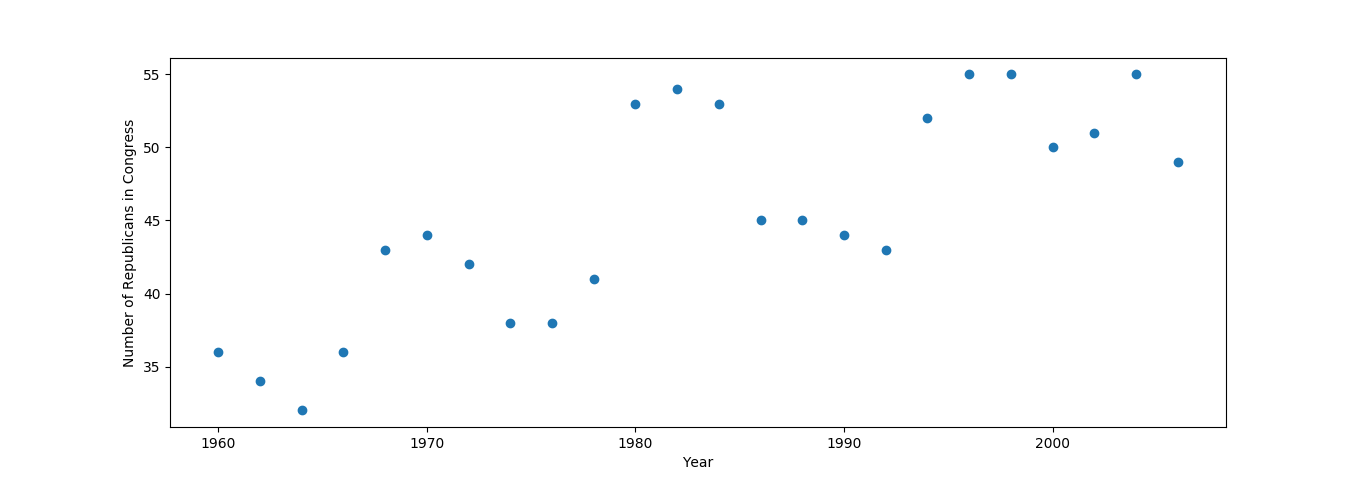
\includegraphics[width=.7\textwidth]{data/year-republicans}
\end{center}

\begin{center}
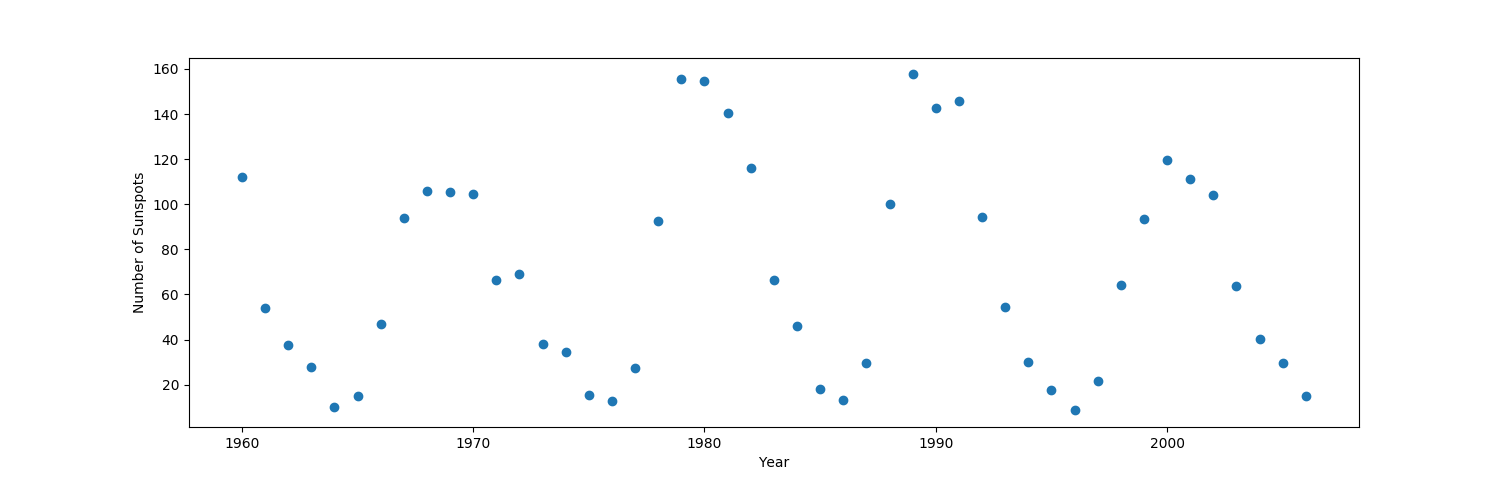
\includegraphics[width=.7\textwidth]{data/year-sunspots}
\end{center}

(Data Source: \url{http://www.realclimate.org/data/senators_sunspots.txt})\\

\begin{enumerate}

\item Implement basis function regression with ordinary least squares for
years vs. number of Republicans in the Senate. Some sample Python code
is provided in \verb|linreg.py|, which implements linear regression.
Plot the data and regression lines for the simple linear case, and for
each of the following sets of basis functions (use basis (b) only for Republicans v. Years, skip for Sunspots v. Years):
\begin{enumerate}
  \item[(a)] $\phi_j(x) = x^j$ for $j=1, \ldots, 5$ 
    \item[(b)] $\phi_j(x) = \exp{\frac{-(x-\mu_j)^2}{25}}$ for $\mu_j=1960, 1965, 1970, 1975, \ldots 2010$
  \item[(c)] $\phi_j(x) = \cos(x / j)$ for $j=1, \ldots, 5$
  \item[(d)] $\phi_j(x) = \cos(x / j)$ for $j=1, \ldots, 25$
\end{enumerate}

\item In addition to the plots, provide one or two sentences for each with
numerical support, explaining whether you think it is fitting well,
overfitting or underfitting.  If it does not fit well, provide a
sentence explaining why. A good fit should capture the most important
trends in the data.

\item Next, do the same for the number of sunspots vs. number of
Republicans, using data only from before 1985.  What bases provide the
best fit?  Given the quality of the fit, would you believe that the
number of sunspots controls the number of Republicans in the senate?

\end{enumerate}

\end{problem}
\pagebreak
\subsection*{Solution}

Attached in the files is "linreg.py" which I just directly modified to produce these graphics and errors. Below are the graphs, errors, and analysis in order from 1. (a)(b)(c)(d) 3. (a)(c)(d).

\begin{figure}[h]
\centering
\includegraphics[width=9cm]{screenshots/2a.png}
\end{figure}

\bigskip \noindent The sum of squares error for this graph is 212.4388959301186.

\bigskip \noindent I think the graph is a good fit. It captures the overall pattern that more republicans are in congress over the years, without paying much attention to the random noise (that appears to be sinusoidal?). 

\begin{figure}[h]
\centering
\includegraphics[width=9cm]{screenshots/2b.png}
\end{figure}

\bigskip \noindent The sum of squares error for this graph is 27.136548308359743.

\bigskip \noindent I think this graph is a fairly good fit, maybe a bit overfitting. It seems to notice a different pattern that's not strictly "increasing" like the one in (a), rather it picks up on the weird sinusoidal nature of the dots. However, it doesn't seem to be TOO affected by noise as you can see near the end, the model doesn't go crazy trying to fit itself to every data point. 

\newpage

\begin{figure}[h]
\centering
\includegraphics[width=9cm]{screenshots/2c.png}
\end{figure}

\bigskip \noindent The sum of squares error for this graph is 541.4044279933597.

\bigskip \noindent I think the graph is underfitting. It looks closer to a general mean than an actual curve fit ... a lot of points are way off from the regression line. The error value is also very high.

\begin{figure}[h]
\centering
\includegraphics[width=9cm]{screenshots/2d.png}
\end{figure}

\bigskip \noindent The sum of squares error for this graph is 19.533002674775688.

\bigskip \noindent I think the graph is overfitting. The error is low (which in this case is a bad thing). It looks very similar to the graph in (b) that i said was a somewhat well fit, the issue is that this one seems to adjust too much to noise: except for the last dot, it tries to touch every single data point (and you see the model start to curve sharply downwards, so maybe it even hits the last point as well). Adjusts too much to random noise whereas (b) was tamer in the last section.

\newpage

\begin{figure}[h]
\centering
\includegraphics[width=9cm]{screenshots/2a1.png}
\end{figure}

\bigskip \noindent The sum of squares error for this graph is 175.6139678870893.

\bigskip \noindent I think the graph is an alright fit. The general trend in the datapoints point towards a positive correlation between sunspots and republicans, which is expressed in the regression. Some noise is amplified, as seen near the 140 sunspots range, but for most of the data the regression appears reasonable. 

\begin{figure}[h]
\centering
\includegraphics[width=9cm]{screenshots/2c1.png}
\end{figure}

\bigskip \noindent The sum of squares error for this graph is 187.5533788908371.

\bigskip \noindent I think the graph is overfitting. There is a ton of random noise between the dots, with curves up and down that don't make sense, despite not even being that accurate and hitting the dots. Seems like the data points are very influential in the shape of the model. 

\newpage

\begin{figure}[h]
\centering
\includegraphics[width=9cm]{screenshots/2d1.png}
\end{figure}

\bigskip \noindent The sum of squares error for this graph is 4.465331376785433e-25.

\bigskip \noindent I think the graph is overfitting. The loss is too small, the regression line predicts some really weird patterns caused by the fact that it wants to fit every single data point. Seems out of place and too adjusted to the noise.

\bigskip \noindent For question 3, I believe that basis (A) provides the best fit (the other two were overfitting). Given the quality of the fits, I would not believe that the number of sunspots controls the number of republicans in the senate: even with the best basis graph, the model seemed strange and didn't seem to capture the data well (losses were high).


%%%%%%%%%%%%%%%%%%%%%%%%%%%%%%%%%%%%%%%%%%%%%
% Problem 4
%%%%%%%%%%%%%%%%%%%%%%%%%%%%%%%%%%%%%%%%%%%%%
\newpage
\begin{problem}[Administrative]
\leavevmode
\begin{itemize}
    \item Name: Miles Wang 
    \item Email: mileswang@college.harvard.edu
    \item Collaborators: Emily Jia, Lily Zhao, Anubha Srivastava, Lora Stoyanova
    \item Approximately how long did this homework take you to complete (in hours): 40
\end{itemize}
\end{problem}


\end{document}
